%  article.tex (Version 3.3, released 19 January 2008)
%  Article to demonstrate format for SPIE Proceedings
%  Special instructions are included in this file after the
%  symbol %>>>>
%  Numerous commands are commented out, but included to show how
%  to effect various options, e.g., to print page numbers, etc.
%  This LaTeX source file is composed for LaTeX2e.

%  The following commands have been added in the SPIE class 
%  file (spie.cls) and will not be understood in other classes:
%  \supit{}, \authorinfo{}, \skiplinehalf, \keywords{}
%  The bibliography style file is called spiebib.bst, 
%  which replaces the standard style unstr.bst.  

\documentclass[]{spie}  %>>> use for US letter paper
%%\documentclass[a4paper]{spie}  %>>> use this instead for A4 paper
%%\documentclass[nocompress]{spie}  %>>> to avoid compression of citations
%% \addtolength{\voffset}{9mm}   %>>> moves text field down
%% \renewcommand{\baselinestretch}{1.65}   %>>> 1.65 for double spacing, 1.25 for 1.5 spacing 
%  The following command loads a graphics package to include images 
%  in the document. It may be necessary to specify a DVI driver option,
%  e.g., [dvips], but that may be inappropriate for some LaTeX 
%  installations. 
\usepackage[]{graphicx}
\newcommand{\figsimple}{10cm} %setea el tamaño de todas las figuras

\title{Confocal Raman thermometer for microfluidic devices} 

%>>>> The author is responsible for formatting the 
%  author list and their institutions.  Use  \skiplinehalf 
%  to separate author list from addresses and between each address.
%  The correspondence between each author and his/her address
%  can be indicated with a superscript in italics, 
%  which is easily obtained with \supit{}.

\author{Guillermo D. Brinatti Vazquez\supit{a,b}, Oscar E. Martínez\supit{a,b} and Juan Martín Cabaleiro\supit{a,c,d}
\skiplinehalf
\supit{a}Consejo Nacional de Investigaciones Científicas y Técnicas, Argentina. \\
\supit{b}Laboratorio de Fotónica, Facultad de Ingeniería, Universidad de Buenos Aires, Argentina.\\
\supit{c}Laboratorio de Fluidodinámica, Facultad de Ingeniería, Universidad de Buenos Aires, Argentina.\\
\supit{d}Laboratorio de Micro y Nanofluídica y Plasma, UdeMM, Buenos Aires, Argentina.
}

%>>>> Further information about the authors, other than their 
%  institution and addresses, should be included as a footnote, 
%  which is facilitated by the \authorinfo{} command.

\authorinfo{Further author information: (Send correspondence to A.A.A.)\\A.A.A.: E-mail: aaa@tbk2.edu, Telephone: 1 505 123 1234\\  B.B.A.: E-mail: bba@cmp.com, Telephone: +33 (0)1 98 76 54 32}
%%>>>> when using amstex, you need to use @@ instead of @
 

%%%%%%%%%%%%%%%%%%%%%%%%%%%%%%%%%%%%%%%%%%%%%%%%%%%%%%%%%%%%% 
%>>>> uncomment following for page numbers
% \pagestyle{plain}    
%>>>> uncomment following to start page numbering at 301 
%\setcounter{page}{301} 
 
  \begin{document} 
  \maketitle 

%%%%%%%%%%%%%%%%%%%%%%%%%%%%%%%%%%%%%%%%%%%%%%%%%%%%%%%%%%%%% 
\begin{abstract}
A confocal Raman microscopy technique has been designed and demonstrated that measures the
temperature rise and profile in microfluidic devices. The system is based in the deformation of the water
Raman peak assigned to the O-H stretching at 3400~cm$^{-1}$ that occurs with temperature keeping an
isosbectic point at 3425~cm$^{-1}$. Hence two photon counting detectors that sample the Raman emission at
each side of the isosbectic point are used to monitor the water temperature. Using a confocal detection
scheme the spatial resolution of a confocal microscope can be obtained to map the temperature profile
within small microfluidic structure in a noninvasive manner. The differential signal between the two
channels normalized by the added signals has a linear dependence with temperature that yields a
sensitivity of 0.8~K using a 1s integration time and a count rate per channel of $1.5\cdot 10^5$ . The pump laser used had a 405~nm wavelength and 20~mW average power. The confocal collection was performed by a
single mode optical fiber and the explored volume was of about 40~$\mu$m$^3$ . The temperature rise in
electrotrofluidic devices was studied showing that the temperature increase depended on the power
used to move the sample along the channel (electroosmotic flow) and the particular design and
structure of the device that determines the heat dissipation mechanism. The scheme proved useful to
evaluate and prevent detrimental temperature effects with the advantage that no specific temperature
sensitive particle needs to be added to the fluid, and has the additional virtue of allowing spatial scans in
3D.
\end{abstract}

%>>>> Include a list of keywords after the abstract 

\keywords{Manuscript format, template, SPIE Proceedings, LaTeX}

%%%%%%%%%%%%%%%%%%%%%%%%%%%%%%%%%%%%%%%%%%%%%%%%%%%%%%%%%%%%%
% \label{} allows reference to this section
\section{INTRODUCTION}

Electroosmotic pumping and electrophoresis are the main strategies to move liquid or species in microfluidic devices  \cite{hunter2001,lyklema1995}. In any of the latter, an electric current is passed through the liquid, resulting in Joule heat dissipation on the medium. This will cause a temperature rise on the device that will depend on its dissipation efficiency. As these techniques are often used in biological applications \cite{tian2008} an undesired temperature rise could change drastically the experiment evolution or even make it fail. Also, as the electroosmotic and electrophoretic mobility are a function of temperature \cite{tang2006} a poor thermal control could lead to an unexpected pumping behavior. This is why temperature monitoring and dissipation efficiency characterization are of great importance in the field. The readers are referred to the reviews by Xuan~\cite{xuan2008} and Cetin and Li~\cite{cetin2008} for a deeper description of joule heating in electrokinetic flows. 

With this purpose different techniques were introduced to measure temperature inside microchannels. A common approach is to make use of thermal properties in fluorescent dyes to indirectly measure temperature from fluorescence imaging \cite{tang2006,ross2001,erickson2003,dye1,dye2}. This involves introducing an additional compound in the flow that could modify chemical reactions occurring inside the microchannel, making the method unsuitable for online monitoring. Moreover, the measurement ``integrates'' the temperature in the channel height, not allowing for the measurement of temperature profiles normal to the channel bottom. 

Walrafen et al \cite{walrafen1} discovered that the infrared spectrum of water shows temperature dependent qualities and measured the existence of an isosbestic point around 3425~$\mathrm{cm^{-1}}$. This molecular property can be sensed using Raman Scattering to get a temperature dependent signal that is intrinsic of water. This method was proposed and proved useful in microchannels \cite{raman1,raman2,raman3} where an epi-illumination microscope was adapted to measure the Raman spectrum by exciting the water with a visible laser. Temperature is then recovered by analizing these spectra. As water absorption is low in visible wavelenghts \cite{absorption} this method proved to be non-invasive.

In this work we propose a device which improves from previous attempts by improving spatial resolution using a confocal collection scheme and by increasing the acquisition speed by splitting the spectrum in the isosbestic point and sending each portion to an independent detector. This results in a device capable of mapping temperature in three dimensions, allowing to study the thermal properties of the flow and the different surfaces of the microfluidic device. Also, the method shown a result where a correlation between type of flow and temperature is found. Additionally, a dark field illumination scheme is used to get scattering or fluorescence images of the sample at the same time temperature measurements take place.

\section{EXPERIMENT}

The device proposed to measure temperature inside microfluidic devices is depicted in figure \ref{fig:setup}. A 150~mW laser diode emitting at 405~nm is used as excitation beam. The light is coupled to a single mode (SM) optical fiber (using aspheric lenses L0 and L1) acting as spatial filter. The light exiting the fiber is collimated by a triplet lens (L2) and sent into the microscope by reflecting in a long pass dichroic mirror (420 LP) centered in 420~nm. A short pass filter (450 SP) is used to block any light in the detection band. The light then reflects in a second long pass dichroic mirror (505 LP) centered in 505~nm and then is focused in the sample using a 40X 0.95 NA microscope objective. The total power in the sample at 405~nm is around 25~mW. 

The Raman scattering (around 470~nm) collected by the same objective is separated from the excitation path as it is transmitted in the first dichroic mirror. The light is then couplet to a Multi mode (MM) optical fiber (10~$\mu m$ core diameter) using a 10X 0.28 NA microscope objective. This step gives the microscope confocal resolution as the light coming from outside the confocal volume will have a poor coupling efficiency. The other end of the optical fiber is sent to an opaque box containing the detection part of the setup, where the light is collimated and directed to a 300 lines/mm diffraction grating (DG). An achromatic lens is used to focus the diffracted light into a D shaped mirror (DM) mounted in a translation stage used to split the spectrum at the isosbestic point. Each new light path is then directed to a independent photon counter (PMT A and PMT B) for detection. A lens (LA and LB) and a longpass filter (FA and FB) are used before the detector to get an image of the plane of DM and to remove light at the laser wavelenght. The voltage pulses coming from the detectors are registered by a on board, two channel, 32 bit counter in a PC.  

\begin{figure}[h!]
\centering
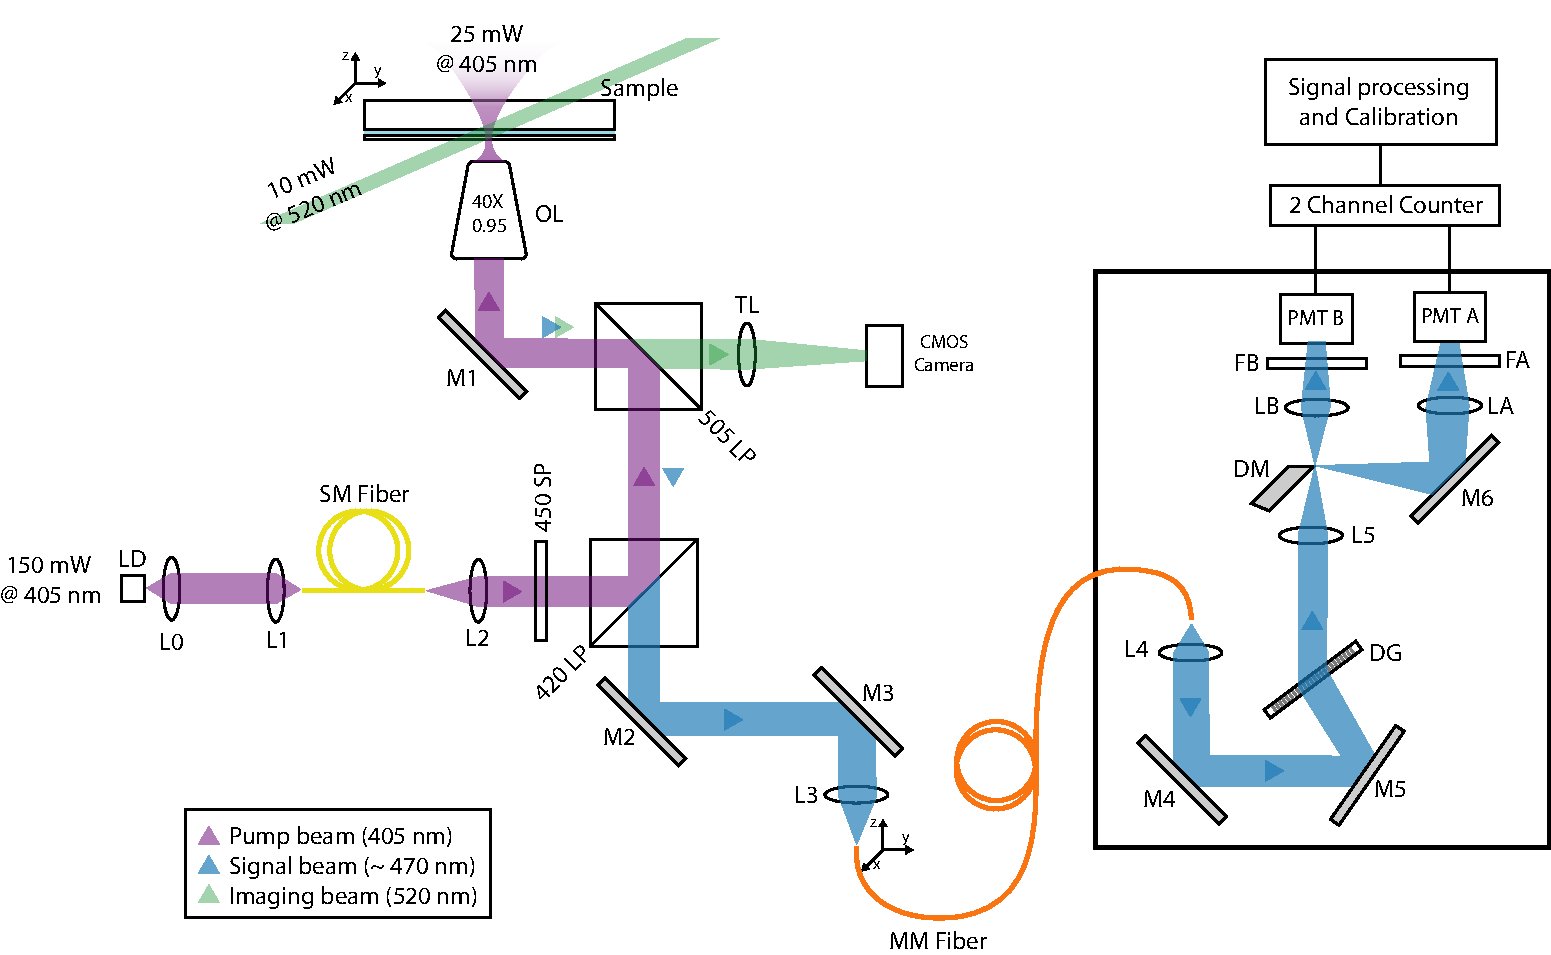
\includegraphics[width =\textwidth]{figs/setup.pdf}
\caption{Schematic representation of the microscope used for Raman thermometry. A 150 mW laser diode emitting in 405~nm (LD) is used as excitation beam. A single mode (SM) fiber is used as a spatial filter before focusing the beam on the sample using a 40X 0.95 NA microscope objective. A dichroic mirror centered in 420~nm is used to separate the collected Raman emission (centered around 470~nm) which is focused in a Multi mode (MM) fiber which grants confocal resolution. The output of the fiber is sent to a spetially made spectroemeter which split the spectrum at the isosbestic point and sent each channel to a independent photon counter device. Signal processing and calibration is made in a PC. A 10~mW, 520~nm beam is used to illuminate the sample in a dark field scheme. This results in a scattering image of the sample in a CMOS camera.
\label{fig:setup}}
\end{figure}

The sample is also illuminated in a dark field scheme using a 10~mW laser beam emitting at 520~nm. The scattering or fluorescence produced by this beam is then separated from the pump and signal beam as it is transmitted trough 505~LP. A 100~mm tube lens is used to get a image of the sample on a CMOS camera. This is used to set the sample in place and to track particles incorporated in the liquid in order to measure flow velocity. This can be used to study the flow inside the microchannel without interfering with the signal path if low particle concentrations are used to avoid fluorescence signals excited by the pump beam that could lay in the Raman spectrum. As the confocal volume is small, the probability of such event is also small if low concentrations are used.   

As the collection is confocal a three dimensional characterization of the sample is possible with the proper scanning mechanism. In this application we choose to use a three axis motorized stage to move the sample in all dimensions. A galvo mirror design is also possible in applications where speed is required. Two angular degrees of freedom are used in the sample holder in order to set the detection plane parallel to the microchannels. The axial resolution achieved with the setup is of 9~$\mu \mathrm{m}$ resulting in a collection volume of around 40~$\mu \mathrm{m}^3$ with a photon count rate of $1.5 \cdot 10^5$~s$^{-1}$ on each detector.  

Microfuidics chips were made by polydimethylsiloxane (PDMS) replication of a Silicon-SU8 master. The PDMS microchannels produced were sealed with 150~$\mu$m thick glass coverslips. To improve the superficial bond between glass and PDMS, both parts were exposed to microwave air plasma and then gently held together. The plasma step is not mandatory due to the low manometric pressure into the channel, however plasma bonding allows for easier manipulation of the chip as the bonding is permanent. Plastic round reservoirs (made by cutting 10 ml plastic syringes, Diameter $\sim$ 16~mm) were attached to both ends of the straight microchannels. The channels were filled with a 5000~$\mu$S/cm KCl solution. Polystyrene microspheres 1~$\mu$m in diameter were incorporated to the fluid in a low concentration in order to set the proper initial condition (zero fluid velocity) before the electric field is turned on. This was achieved by detecting the scattering of the particles on the camera and tracking their positions. A power supply delivering up to 1~kV is used to establish the flow.
 
\section{RESULTS AND DISCUSSION}

%\begin{figure}[h!]
%\centering
%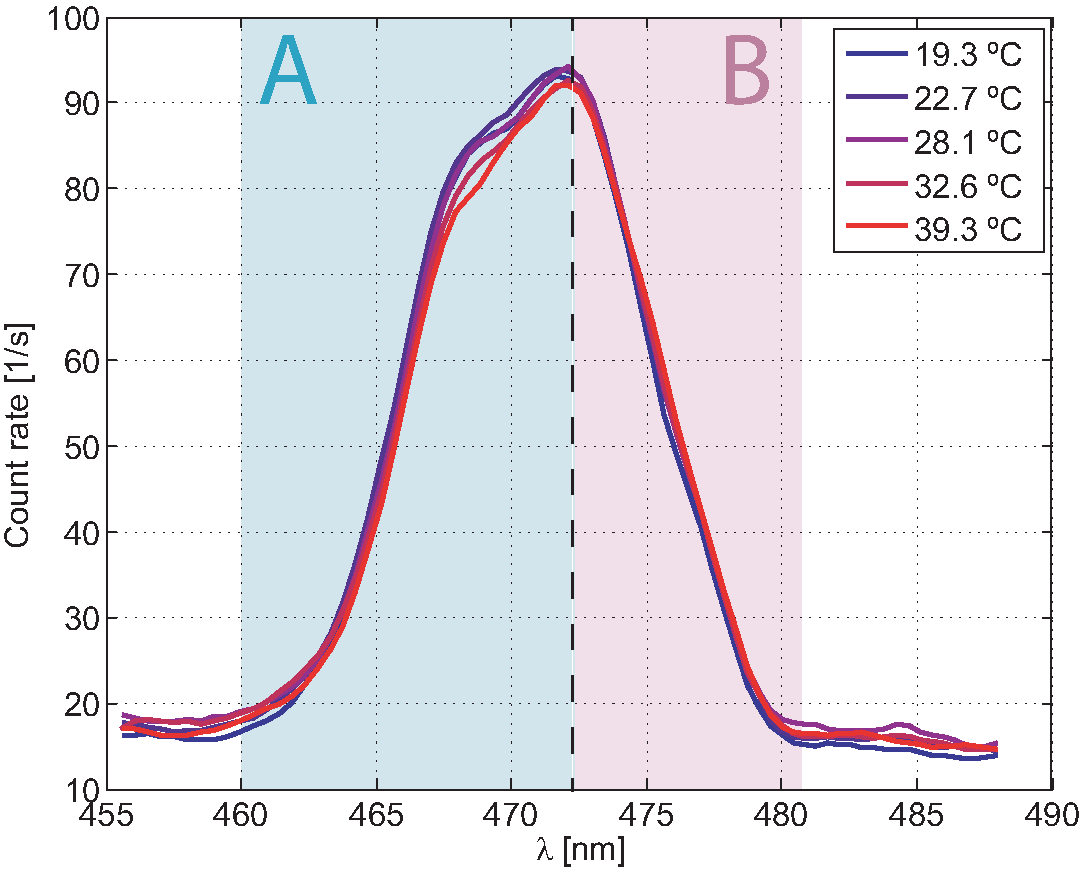
\includegraphics[width=\figsimple]{figs/spectra.pdf}
%\label{}
%\caption{}
%\end{figure}

First we start by showing a calibration for the technique in figure \ref{fig:calibration}. This was made by using a temperature controlled water cell in the sample plane. By measuring simultaneously the temperature of the cell and the water using Raman thermometry we obtain a linear calibration. The spread of the data points around the linear fit result in a resolution of 0.8~K using a integration time of 1 s. All the measurements in this article were performed with this integration time. 

\begin{figure}[h!]
\centering
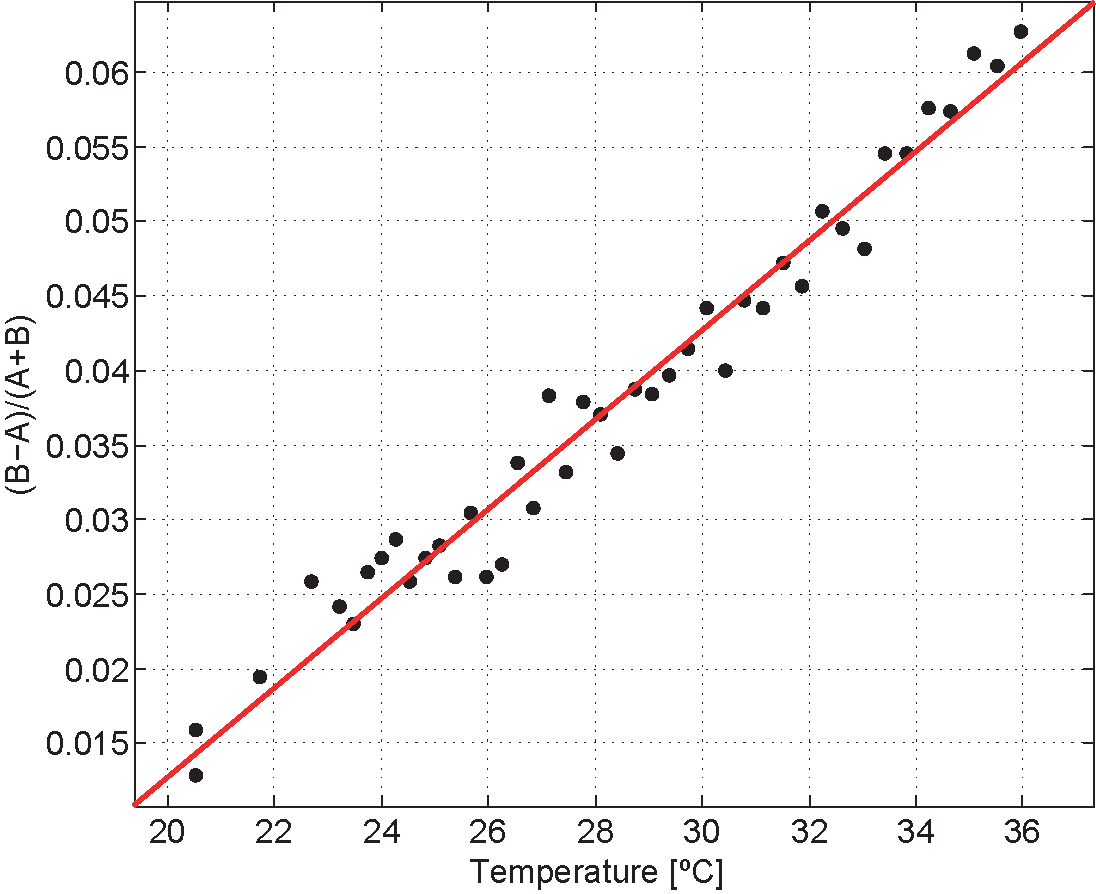
\includegraphics[width=\figsimple]{figs/calibration.pdf}
\caption{Temperature dependent signal as a function of temperature. A linear fit of the data results in a proper calibration. A resolution of 0.8~K is achieved with a 1~s integration time. 
\label{fig:calibration}}
\end{figure}

\begin{figure}[h!]
\centering
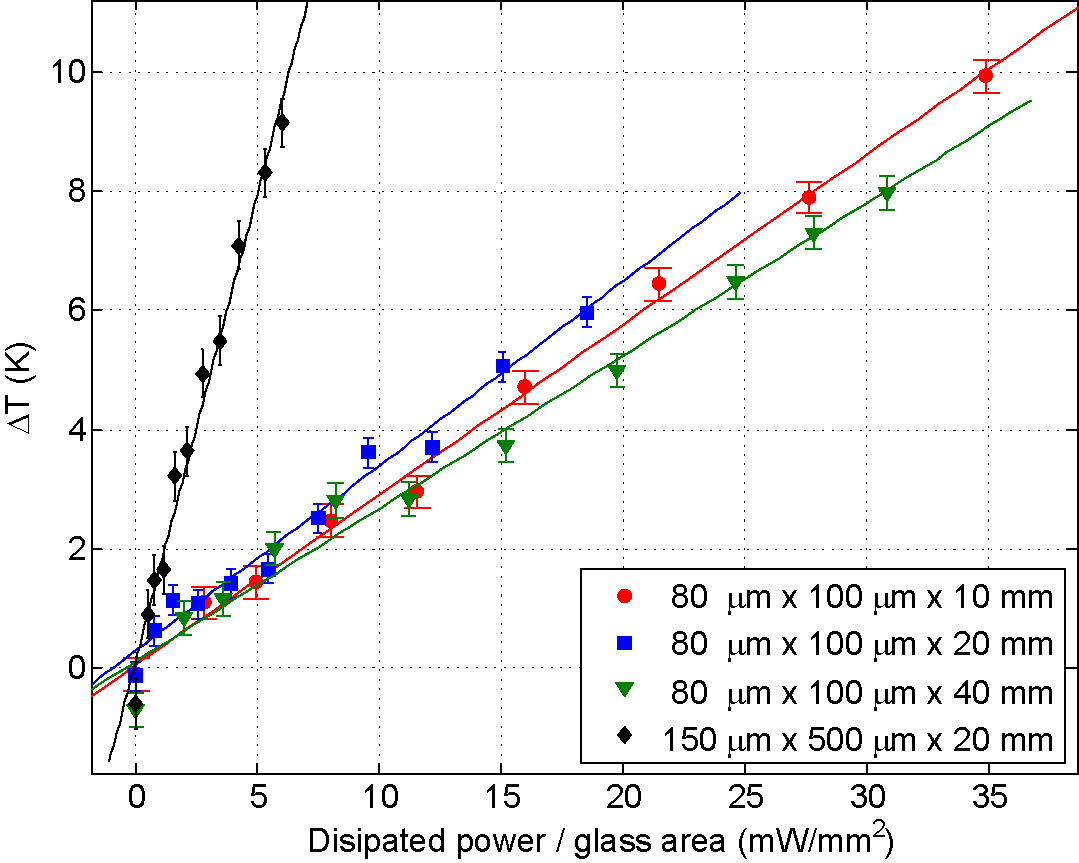
\includegraphics[width=\figsimple]{figs/rectas.pdf}
\caption{Temperature rise versus dissipated power per glass area for microchannels of different geometry. A linear fit is shown for each data set.  \label{fig:rectas}}
\end{figure}


The temperature rise at the center of each microchannel was measured using the technique as a function of the Joule heat dissipated in the device. The result of this experiment is shown in figure \ref{fig:rectas} where temperature rise is plotted against dissipated power per unit glass area for different channel geometries. A linear fit is displayed for each data set. For the three channels with 80~$\mu$m height we can see that the slope of the linear feat is fairly similar. This indicates that the glass floor of the device is the main dissipation mechanism, independently of the lenght of the channel. For the taller 150~$\mu$m channel we see a drastic change in its slope, indicating a different heat flow in the channel.  

As the technique is confocal 3D spatial scans are possible. In figure \ref{fig:vertical} a vertical scan from the center of the channel to the glass surface is shown. The same experiment was repeated for the smaller channels resulting in a constant temperature profile, in good agreement with theory and previous experiments. In the case of the wider channel, two different temperatures are observed separated by an abrupt change. The center of the channel about 3 K hotter than the water surrounding the base of the channel. 

\begin{figure}[h!]
\centering
\includegraphics[width=\figsimple]{figs/vertical_raro.pdf}
\caption{Temperature as a function of height from the center (left side) to the glass floor of the channel (right side) with dimensions 150~$\mu$m x 500~$\mu$m x 20~mm (height x base x lenght).\label{fig:vertical}}
\end{figure}

\begin{figure}[h!t!b!]
\centering
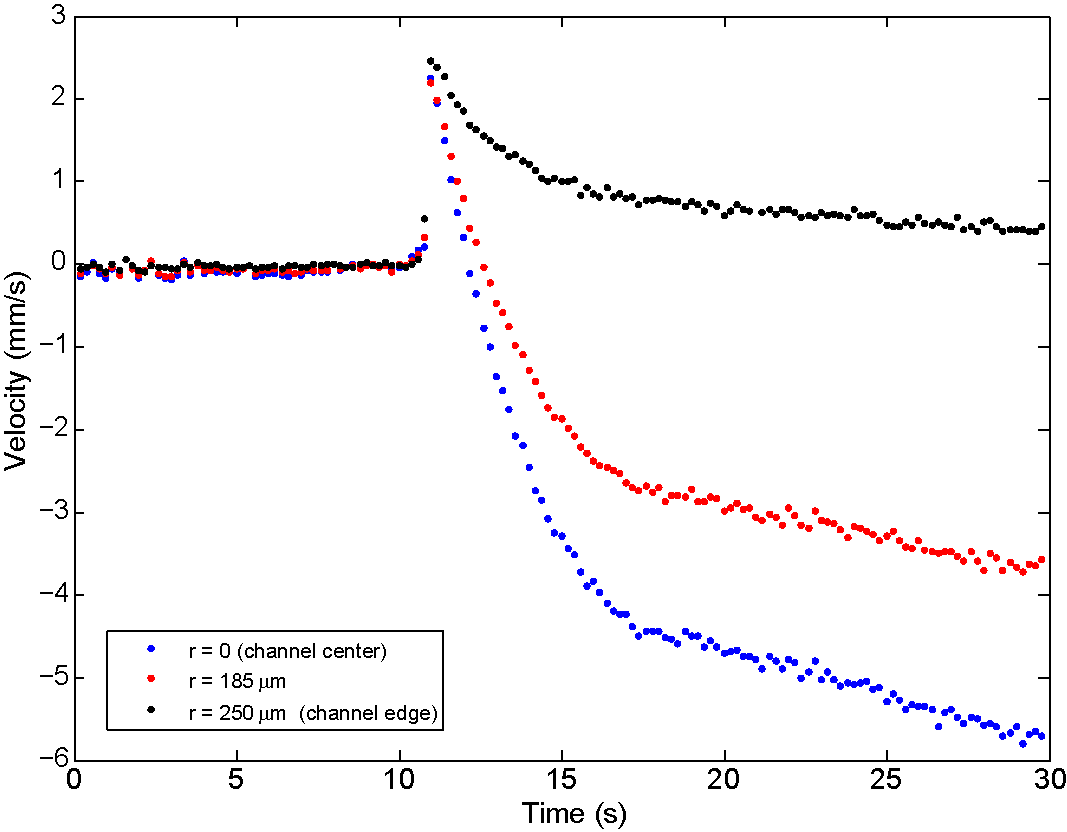
\includegraphics[width=\figsimple]{figs/PIV2D.pdf}
\caption{PIV measurement for the 150~$\mu$m x 500~$\mu$m x 20~mm microchannel for three different positions form the center to the edge of the device. \label{fig:piv}}
\end{figure}
For a complete characterization of the channels a Particle Imaging Velocimetry (PIV) measurement was independently performed in the same conditions for each device. Figure \ref{fig:piv} shows the results of this experiment for the channel exhibiting a different behaviour. The PIV corresponding to the small channels show a constant \textit{plug type} flow in all the measuring interval. For this channel a an initial planar flow is observed when electric field is turned on around $t = 11$~s, but is rapidly lost due to the pressure difference generated between the reservoirs. This results in a parabolic flow in opposite direction to the initial flow with a maximum at the center of the channel. With this information, results shown in figure \ref{fig:vertical} can be understood as the flow is bidirectional. Each stream is flowing without exchanging mass with its counterpart and develop a different temperature, with a sharp step at the interface.
 


\section{Conclusions}

A novel technique to measure temperature in microfluidic devices is shown. The method uses the dependency on temperature of the Raman spectrum of water and improves from previous implementations that the collection is confocal, giving a improved three dimensional resolution, and the detection is made using a pair of photon counters which improves measuring time as is not necessary to measure the whole spectrum in each position. The technique shows good agreement with results from other methods and theoretical calculations \cite{erickson2003}. We also show that the device is useful to characterize microfluidic chips, giving useful information for the election of dimensions and construction materials in the design stage. 

The technique also shows a thermal behavior never reported before when a bidirectional flow is observed. Each flow develop its own temperature and a sharp gradient is observed at the interface. This was correlated with PIV measurements performed independently in the same conditions.


\bibliography{bibliography}   %>>>> bibliography data in report.bib
\bibliographystyle{spiebib}   %>>>> makes bibtex use spiebib.bst

\end{document} 







